\documentclass[11pt,a4paper]{article}

% ---------- packages ----------
\usepackage[utf8]{inputenc}
\usepackage[T1]{fontenc}
\usepackage{lmodern}
\usepackage[a4paper,margin=2.4cm]{geometry}
\usepackage{amsmath,amssymb}
\usepackage{graphicx}
\usepackage{booktabs}
\usepackage{caption}
\usepackage{subcaption}
\usepackage{xcolor}
\usepackage{listings}
\usepackage{tikz}
\usetikzlibrary{shapes.geometric,arrows.meta,positioning,fit,backgrounds}
\usepackage{enumitem}
\usepackage{microtype}
\usepackage[hidelinks]{hyperref}
\usepackage{titlesec}

\setlength{\parskip}{0.45em}
\setlength{\parindent}{0pt}
\titleformat{\section}{\large\bfseries}{\thesection.}{0.6em}{}
\titleformat{\subsection}{\normalsize\bfseries}{\thesubsection}{0.6em}{}

% ---------- code style ----------
\definecolor{codebg}{rgb}{0.97,0.97,0.97}
\definecolor{codekw}{rgb}{0.10,0.10,0.65}
\definecolor{codecm}{rgb}{0.30,0.55,0.30}
\definecolor{codestr}{rgb}{0.65,0.15,0.15}
\lstdefinestyle{py}{
  language=Python,
  backgroundcolor=\color{codebg},
  basicstyle=\ttfamily\scriptsize,
  keywordstyle=\color{codekw}\bfseries,
  commentstyle=\color{codecm}\itshape,
  stringstyle=\color{codestr},
  numbers=left, numberstyle=\tiny\color{gray}, numbersep=6pt,
  frame=single, rulecolor=\color{gray!40},
  breaklines=true, showstringspaces=false, tabsize=2,
  columns=fullflexible, captionpos=b,
}

\title{\vspace{-1.0cm}\textbf{Predicting Ethereum Gas Prices Using Deep Learning:\\
An LSTM-Based Time-Series Forecasting Approach}\\[0.4em]
\large COM4532 --- Blockchain Technologies \\ Final Project Report}
\author{Boran \"Omer Do\u{g}an (21290594) \and Arif Erdem Orhan (21290337) \and Furkan \c{C}a\u{g}atay \"Ozbek (21290216)}
\date{June 2026}

\begin{document}
\maketitle
\thispagestyle{empty}

\begin{abstract}
\noindent
Ethereum gas fees are volatile and difficult to anticipate, forcing users either to overpay
or to risk transactions stalling. This project formulates next-day gas-price forecasting as a
multivariate time-series regression problem and attacks it with a two-layer Long Short-Term
Memory (LSTM) network trained on $\sim$878 days of post-EIP-1559 on-chain data collected from
Etherscan's public chart exports. Nine input features --- six on-chain metrics, an engineered
day-over-day price delta, and a cyclically encoded day-of-week signal --- are fed to the model
through a 30-day sliding window. We compare the LSTM against four baselines (Na\"ive, 7-day
Simple Moving Average, ARIMA, and XGBoost) under a strict chronological train/validation/test
split, and we interpret the model with SHAP. On the held-out test set (4 Oct -- 30 Dec 2023) the
LSTM attains MAE $=9.13$, RMSE $=11.37$, MAPE $=30.2\%$, and $R^2=0.458$. The day-of-week
feature improves every LSTM metric and SHAP ranks it as the most influential non-price feature.
A central, honestly reported finding is that the Na\"ive ``tomorrow $=$ today'' baseline remains
the strongest predictor ($R^2=0.751$): daily average gas price behaves close to a random walk,
which is itself the scientifically interesting conclusion of the study.
\end{abstract}

\tableofcontents
\newpage

% ============================================================
\section{Introduction and Background}
% ============================================================

\subsection{Description of the Problem}
Ethereum is a permissionless, open-source blockchain platform for executing decentralized
applications (dApps) and smart contracts. Every operation performed by the Ethereum Virtual
Machine is metered in a unit called \emph{gas}, which both rations scarce computational
resources and protects the network from spam. Users pay for the gas their transactions consume
in Ether (ETH). Because block space is finite while demand fluctuates wildly, the price a user
must pay per unit of gas --- the \emph{gas price}, quoted in Gwei ($10^{-9}$ ETH) --- is highly
volatile. During acute demand events such as a high-profile NFT mint or a DeFi liquidation
cascade, gas prices can rise by an order of magnitude within hours.

This volatility translates directly into financial uncertainty. A user who sets the gas price
too low risks having a transaction sit unconfirmed for hours; a user who sets it too high
overpays substantially. The concrete problem addressed by this project is therefore:
\emph{given the recent history of on-chain network metrics, can we forecast tomorrow's average
gas price accurately enough to help users and dApp schedulers plan their transactions?}

\subsection{Motivation}
The economic stakes are large. Aggregated across the network, even small per-transaction
inefficiencies amount to enormous wasted expenditure. A reliable forecast would let a patient
user defer a non-urgent transaction to a cheaper window, and let an automated scheduler (for
example a DeFi rebalancer or an airdrop claimer) submit transactions when fees are low. Unlike
a binary ``high/low'' classifier, a regression model that emits a concrete Gwei estimate can be
fed directly into a wallet's fee field, which is why we adopt a regression formulation.

\subsection{Current Approaches and Their Limitations}
Existing fee estimators embedded in wallets and explorers (MetaMask, Etherscan's gas tracker)
are overwhelmingly \emph{reactive}: they report a weighted average of recently included gas
prices, or an oracle minimum over the last few blocks. These heuristics describe the current
state of the network reasonably well but cannot \emph{anticipate} change. They cannot warn a
user that fees will spike in ten minutes when an NFT collection opens for minting, nor that
waiting an hour will cut fees substantially. What is missing is a \emph{proactive} forecasting
system that learns temporal structure from historical data.

EIP-1559 (London hard fork, August 2021) partially smoothed short-term dynamics by replacing
the first-price auction with a protocol-set \emph{base fee} that adjusts by at most $\pm12.5\%$
per block and is \emph{burned} rather than paid to validators, plus a voluntary \emph{priority
fee} (tip). The base-fee update rule is
\begin{equation}
\mathrm{BaseFee}_{t+1} = \mathrm{BaseFee}_{t}\left(1 + 0.125\cdot
\frac{\mathrm{GasUsed}_t - \mathrm{GasTarget}_t}{\mathrm{GasTarget}_t}\right),
\qquad \mathrm{GasTarget} = \tfrac{1}{2}\,\mathrm{GasLimit}.
\end{equation}
While this makes block-to-block changes smoother, EIP-1559 does \emph{not} eliminate
large-scale volatility driven by demand surges --- anticipating those surges remains an open
problem, which is precisely the gap this project targets.

\subsection{Why Blockchain Technology Is Relevant}
Blockchains are uniquely suited to data-driven analysis: every block, transaction, and fee is
recorded permanently and publicly. This yields a clean, complete, tamper-evident historical
record that would be impossible to obtain for most traditional financial systems. The
relationships between on-chain quantities (congestion, transaction volume, base-fee trajectory)
are strongly non-linear and the price signal is noisy and non-stationary --- exactly the regime
in which simple statistics struggle and sequence models such as LSTMs are expected to help.

\subsection{Blockchain Ecosystem and Data Source}
We restrict attention to the \emph{post-EIP-1559} period (from 5 August 2021 onward) so that the
data reflects a single, consistent fee mechanism and avoids the structural break that mixing
pre- and post-London data would introduce. All data is collected from \textbf{Etherscan's public
chart exports} (CSV ``Download'' buttons), which provide daily-granularity time series for the
whole chain. Five charts are used: average gas price, total daily gas used, average gas limit,
daily transaction count, and ETH/USD price. From these we derive a network-utilization feature,
a day-over-day price delta, and the next-day prediction target. The full study window spans
5 Aug 2021 -- 31 Dec 2023, $\sim$880 daily observations.

% ============================================================
\section{Related Work and Technical Background}
% ============================================================

\subsection{Blockchain Fundamentals}
A blockchain is an append-only ledger replicated across a peer-to-peer network of \textbf{nodes}.
Each node validates and stores blocks; full nodes hold the entire state, while light nodes hold
headers. \textbf{Transactions} are signed messages that transfer value or invoke contract code;
they are gossiped between nodes, ordered into blocks, and finalized by a \textbf{consensus
mechanism}. Since the September 2022 ``Merge,'' Ethereum uses \textbf{Proof-of-Stake}: validators
stake ETH and are pseudo-randomly selected to propose and attest blocks, replacing the
energy-intensive Proof-of-Work mining that preceded it. This transition is visible in our data
(Section~5) as a discontinuity in the per-day gas-utilization series around mid-September 2022.

\subsection{Smart Contracts, Gas, and DeFi}
\textbf{Smart contracts} are programs stored on-chain and executed deterministically by every
node in the EVM. Because execution consumes the network's shared resources, each EVM opcode has
a fixed \textbf{gas} cost; the transaction's sender pays $\text{gas used}\times\text{gas price}$.
\textbf{Decentralized Finance (DeFi)} --- lending protocols, automated market makers, derivatives
--- generates a large share of on-chain activity and is a primary driver of demand spikes:
liquidation cascades and arbitrage races flood the mempool and bid up gas prices. The
\textbf{day-of-week} effect we exploit later is partly explained by DeFi and trading activity
concentrating on weekdays.

\subsection{The Mempool and Fee Market}
Before inclusion, transactions wait in each node's \textbf{mempool} (the pool of pending,
unconfirmed transactions). Block proposers select transactions to maximize revenue, so when the
mempool is congested the effective price of inclusion rises. The size and composition of the
mempool are therefore leading indicators of imminent fee movements --- a signal our daily,
aggregated dataset cannot see, which we flag as a key avenue for improvement (Section~6.3). Under
EIP-1559 the price a transaction pays decomposes into the burned base fee plus a priority tip;
Etherscan's ``average gas price'' aggregates the realized total over all transactions in a day.

\subsection{Blockchain Analytics}
\textbf{Blockchain analytics} is the practice of extracting insight from on-chain data ---
clustering wallets, detecting anomalies/fraud, labeling entities, or, as here, \emph{forecasting}
network quantities. Analytics tasks are commonly categorized as classification, clustering,
anomaly detection, or prediction; our project is squarely a \emph{prediction} task. The analyzed
entities are aggregated daily \emph{block} and \emph{transaction} statistics rather than
individual wallets or tokens, a deliberate scope choice that trades fine-grained resolution for a
tractable, fully reproducible dataset.

\subsection{Machine Learning Background}
\textbf{Time-series regression.} We predict a continuous scalar (tomorrow's Gwei price) from a
window of past observations, so the natural error metrics are MAE, RMSE, MAPE, and $R^2$
(Section~5).

\textbf{LSTM networks.} Recurrent neural networks process sequences but suffer from
vanishing/exploding gradients over long horizons. The Long Short-Term Memory cell
(Hochreiter \& Schmidhuber, 1997) solves this with a gated memory cell:
\begin{align}
f_t &= \sigma(W_f\,[h_{t-1},x_t] + b_f), &
i_t &= \sigma(W_i\,[h_{t-1},x_t] + b_i), \\
\tilde{C}_t &= \tanh(W_C\,[h_{t-1},x_t] + b_C), &
C_t &= f_t \odot C_{t-1} + i_t \odot \tilde{C}_t, \\
o_t &= \sigma(W_o\,[h_{t-1},x_t] + b_o), &
h_t &= o_t \odot \tanh(C_t),
\end{align}
where $\sigma$ is the logistic sigmoid and $\odot$ is the Hadamard product. The forget gate
$f_t$, input gate $i_t$, and output gate $o_t$ let the network selectively retain or discard
information across many time steps, which is what makes LSTMs effective at capturing both slow
seasonal rhythms and fast event-driven spikes in gas prices.

\textbf{XGBoost.} Gradient-boosted decision trees (Chen \& Guestrin, 2016) build an additive
ensemble of shallow trees that greedily fit the residuals of the current model. XGBoost is a
strong tabular baseline and provides exact feature attributions through tree-path methods, which
we use for interpretation.

\textbf{ARIMA.} The AutoRegressive Integrated Moving Average model is the classical statistical
benchmark for univariate forecasting; it combines autoregression, differencing for stationarity,
and a moving-average error term.

\textbf{SHAP.} SHapley Additive exPlanations assign each feature a contribution to an individual
prediction, grounded in cooperative game theory, giving a principled, model-agnostic notion of
feature importance.

\subsection{Related Studies}
Werner et al. (2020), \emph{Step on the Gas?}, analyze the deficiencies of oracle-style gas
recommenders and motivate data-driven alternatives. Mars et al. (2021) compare machine-learning
approaches (including LSTM) for Ethereum gas-price prediction, and Butt et al. (2023) benchmark
several ML methods for blockchain transaction-fee forecasting. Our work follows this line:
it adopts the LSTM as primary model, but --- crucially --- benchmarks it against simple baselines
under a leakage-free chronological protocol and reports the outcome honestly, including the case
where the deep model does \emph{not} beat the na\"ive predictor.

% ============================================================
\section{System Design / Problem Construction}
% ============================================================

\subsection{Analysis Task}
The task is \textbf{prediction} (regression). Formally, given a sliding window of the past
$w=30$ days of features, predict the average gas price for day $t+1$:
\begin{equation}
X_t = \begin{bmatrix} x_{t-w} \\ x_{t-w+1} \\ \vdots \\ x_{t-1}\end{bmatrix}\in\mathbb{R}^{w\times d},
\qquad \hat{y}_{t+1}\in\mathbb{R}\ \text{(gas price in Gwei)},
\end{equation}
with $w=30$ and $d=9$ features. We deliberately choose regression over classification: a wallet
or scheduler needs a concrete Gwei number, not a coarse ``high/low'' label.

\subsection{Blockchain Data, Sources, and Entities}
\textbf{Data sources.} Five Etherscan public chart CSVs (Table~\ref{tab:features}). \textbf{Entities
analyzed.} Aggregated daily statistics of two on-chain entities: the \emph{block} (gas price, gas
used, gas limit) and the \emph{transaction} (daily count); the ETH/USD price is included as a
market-sentiment proxy. Individual wallets and tokens are out of scope. The choice of daily
granularity is pragmatic: it captures the dynamics relevant to a one-day-ahead forecast while
avoiding the need to process millions of raw transactions.

\subsection{Features Extracted}
\begin{table}[h]
\centering
\caption{The nine input features and their sources.}
\label{tab:features}
\small
\begin{tabular}{@{}llp{6.6cm}@{}}
\toprule
\textbf{Feature} & \textbf{Source / derivation} & \textbf{Rationale} \\
\midrule
Gas\_Price\_Gwei  & \texttt{chart/gasprice}   & The series being forecast (demand for block space) \\
Gas\_Used         & \texttt{chart/gasused}    & Total daily gas consumed (realized demand) \\
Gas\_Limit        & \texttt{chart/gaslimit}   & Average per-block capacity (supply side) \\
Gas\_Utilization  & Gas\_Used $/$ Gas\_Limit  & Congestion proxy (supply/demand balance) \\
Tx\_Count         & \texttt{chart/tx}         & Daily transaction count (raw demand) \\
ETH\_Price\_USD   & \texttt{chart/etherprice} & Market-sentiment proxy \\
Gas\_Price\_Delta & first difference of price & Directional momentum (engineered) \\
DOW\_Sin          & $\sin(2\pi\,\text{dow}/7)$ & Weekly seasonality, cyclic (engineered) \\
DOW\_Cos          & $\cos(2\pi\,\text{dow}/7)$ & Weekly seasonality, cyclic (engineered) \\
\bottomrule
\end{tabular}
\end{table}

The first six features come directly from the proposal. We add two engineered groups. The
\textbf{price delta} (first difference of the gas-price series) encodes whether the network is
currently tightening or loosening. The \textbf{day-of-week} signal is encoded \emph{cyclically}
as a $(\sin,\cos)$ pair rather than as an integer $0\ldots6$, so that Sunday (6) sits adjacent to
Monday (0) instead of being treated as the most distant day; this respects the circular topology
of the week and lets the model represent the documented ``cheaper on weekends'' pattern without
an artificial ordinal jump.

\subsection{Expected Outputs}
The system produces (i) a one-day-ahead gas-price prediction in Gwei for every day in the test
horizon; (ii) a quantitative comparison of the LSTM against four baselines on four metrics;
(iii) SHAP-based explanations identifying which features and which historical lags drive the
predictions; and (iv) serialized model artifacts (\texttt{.keras} and \texttt{.pkl}) plus
CSV/PNG result files.

\subsection{End-to-End Pipeline}
The data-flow proceeds through four stages, summarized below.

\begin{enumerate}[leftmargin=1.4em]
\item \textbf{Collection.} Load the five CSVs, parse dates, coerce numerics, and \emph{outer-join}
on date so no day is silently dropped.
\item \textbf{Preprocessing \& feature engineering.} Forward-/back-fill any missing days,
restrict to the post-EIP-1559 window, auto-convert Wei$\to$Gwei if needed, then derive
utilization, the price delta, the day-of-week encodings, and the next-day target.
\item \textbf{Modeling.} Chronologically split 80/10/10; Winsorize the continuous features at the
99th percentile (caps from \emph{train only}); min-max scale (fit on \emph{train only}); build
30-day windows; grid-search the LSTM; additionally run walk-forward validation.
\item \textbf{Evaluation.} Compute MAE/RMSE/MAPE/$R^2$ for the LSTM and all baselines on the
held-out test set, plot predictions, and compute SHAP explanations.
\end{enumerate}

\begin{figure}[h]
\centering
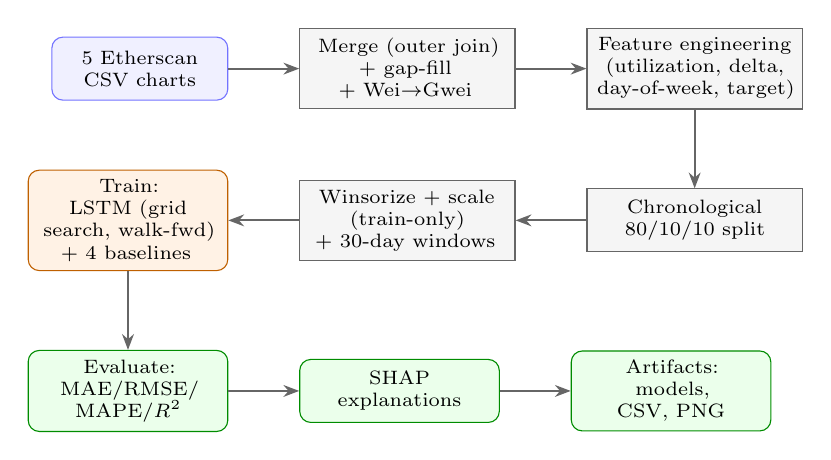
\begin{tikzpicture}[
  node distance=0.55cm and 0.9cm,
  font=\scriptsize,
  src/.style={rectangle, rounded corners, draw=blue!55, fill=blue!6, align=center, minimum height=0.8cm, text width=2.0cm},
  proc/.style={rectangle, draw=black!60, fill=black!4, align=center, minimum height=0.8cm, text width=2.5cm},
  model/.style={rectangle, rounded corners, draw=orange!75!black, fill=orange!10, align=center, minimum height=0.8cm, text width=2.3cm},
  outp/.style={rectangle, rounded corners, draw=green!55!black, fill=green!8, align=center, minimum height=0.8cm, text width=2.3cm},
  arr/.style={-{Stealth[length=2mm]}, thick, black!60}
]
% sources
\node[src] (csv) {5 Etherscan\\ CSV charts};
\node[proc, right=of csv] (merge) {Merge (outer join)\\ + gap-fill\\ + Wei$\to$Gwei};
\node[proc, right=of merge] (feat) {Feature engineering\\ (utilization, delta,\\ day-of-week, target)};
\node[proc, below=1.0cm of feat] (split) {Chronological\\ 80/10/10 split};
\node[proc, left=of split] (prep) {Winsorize + scale\\ (train-only)\\ + 30-day windows};
\node[model, left=of prep] (train) {Train: LSTM (grid\\ search, walk-fwd)\\ + 4 baselines};
\node[outp, below=1.0cm of train] (eval) {Evaluate:\\ MAE/RMSE/\\ MAPE/$R^2$};
\node[outp, right=of eval] (shap) {SHAP\\ explanations};
\node[outp, right=of shap] (art) {Artifacts:\\ models, CSV, PNG};
% arrows
\draw[arr] (csv) -- (merge);
\draw[arr] (merge) -- (feat);
\draw[arr] (feat) -- (split);
\draw[arr] (split) -- (prep);
\draw[arr] (prep) -- (train);
\draw[arr] (train) -- (eval);
\draw[arr] (eval) -- (shap);
\draw[arr] (shap) -- (art);
\end{tikzpicture}
\caption{End-to-end data-flow of the forecasting pipeline, from Etherscan CSV exports to
evaluated models, explanations, and serialized artifacts.}
\label{fig:flow}
\end{figure}

\subsection{Design Decisions That Prevent Data Leakage}
Three deliberate choices keep the evaluation honest, which matters more than headline accuracy in
a non-stationary financial setting:
\begin{itemize}[leftmargin=1.4em]
\item \textbf{Strict chronological split.} The earliest 80\% is training, the next 10\%
validation, the final 10\% test. No shuffling: the model is always evaluated on data strictly
later in time than it was trained on, matching real deployment.
\item \textbf{Train-only statistics.} Both the Winsorization caps and the min-max scaler are fit
exclusively on training rows and then applied to validation/test. No test-set information ever
flows backward.
\item \textbf{Winsorize, don't delete.} Outliers above the 99th percentile are \emph{capped}
rather than removed, so genuine spike days are retained (and contribute to RMSE) but a handful of
$400+$ Gwei days cannot dominate the MSE objective.
\end{itemize}

\subsection{Rationale for the Window Size and Target}
The 30-day lookback $w=30$ is a deliberate trade-off. A longer window gives the LSTM more context
to detect weekly and monthly rhythms (a full month covers $\sim$4 weekly cycles, which is why the
day-of-week feature has lags to exploit), but it also shrinks the number of training windows and
dilutes recent, more relevant information. Shorter windows (e.g.\ 7 days) react faster but cannot
represent monthly structure. Thirty days matches the proposal and is a common choice for daily
financial series. The target is the \emph{level} of the next day's price (a one-step-ahead
forecast), shifted by one row from the feature frame; we discuss in Section~6 why forecasting the
\emph{change} instead would give the learned models a fairer test against the persistence
baseline.

\subsection{Threats to Validity}
Three threats are worth naming explicitly. (i) \emph{Non-stationarity}: the 2021--2022 training
period is far more volatile than the 2023 test period, so a model tuned on the past may
systematically over-predict; we mitigate this with walk-forward validation but cannot remove it.
(ii) \emph{Single market regime}: the entire dataset is post-EIP-1559 and dominated by the
2021--2023 cycle, so conclusions may not transfer to future fee-market changes (e.g.\ blob fees
from EIP-4844). (iii) \emph{Label aggregation}: the daily \emph{average} gas price smooths over
the intra-day urgency spectrum, so even a perfect daily forecast cannot time a transaction within
a day. These threats frame the results in Section~5 and the future work in Section~6.

\subsection{Concrete Split}
After deriving the target and dropping the trailing NaN, the dataset contains \textbf{878 daily
rows}. The chronological split and 30-day windowing yield:
\begin{table}[h]
\centering
\caption{Chronological data split (rows are calendar days; windowed shapes are $(\text{samples},30,9)$).}
\label{tab:split}
\small
\begin{tabular}{@{}lccc@{}}
\toprule
\textbf{Subset} & \textbf{Date range} & \textbf{Calendar days} & \textbf{Windowed shape} \\
\midrule
Train      & 2021-08-05 \ $\to$\ 2023-07-07 & 702 & $(672,30,9)$ \\
Validation & 2023-07-08 \ $\to$\ 2023-10-03 & 88  & $(88,30,9)$ \\
Test       & 2023-10-04 \ $\to$\ 2023-12-30 & 88  & $(88,30,9)$ \\
\bottomrule
\end{tabular}
\end{table}

% ============================================================
\section{Implementation}
% ============================================================
The pipeline is implemented in a single, reproducible Jupyter notebook
(\texttt{gas\_prediction.ipynb}) that auto-detects its runtime (Kaggle / Colab / local) and
auto-locates the CSVs by filename keyword. The experiments reported here were run on Kaggle.

\subsection{Software Libraries}
Python 3, \texttt{pandas}/\texttt{numpy} (data handling), \texttt{scikit-learn} (scaling,
metrics), \texttt{TensorFlow}/\texttt{Keras} (LSTM), \texttt{xgboost} (gradient boosting),
\texttt{statsmodels} (ARIMA), \texttt{shap} (explainability), and
\texttt{matplotlib}/\texttt{seaborn} (figures).

\subsection{Data Collection and Merging}
The five charts are merged with an outer join and gap-filled before filtering. Etherscan
occasionally exports the average gas price in Wei; the notebook detects this from the median and
divides by $10^9$ automatically. In our window, the outer join required \emph{no} forward-filling
(zero missing cells), but the safety net is retained for re-runs over other windows.

\begin{lstlisting}[style=py,caption={Merge, gap-fill, window filter, and Wei$\to$Gwei guard.}]
df = gas_price.join([gas_used, gas_limit, tx_count, eth_price], how='outer')
df = df.ffill().bfill()
df = df[(df.index >= '2021-08-05') & (df.index <= '2023-12-31')]
if df['Gas_Price_Gwei'].median() > 1e6:          # Etherscan sometimes exports Wei
    df['Gas_Price_Gwei'] = df['Gas_Price_Gwei'] / 1e9
\end{lstlisting}

\subsection{Feature Engineering}
\begin{lstlisting}[style=py,caption={Derived, engineered, and target columns.}]
df['Gas_Utilization'] = df['Gas_Used'] / df['Gas_Limit']
df['Gas_Price_Delta'] = df['Gas_Price_Gwei'].diff().fillna(0.0)   # momentum
_dow = df.index.dayofweek                                          # 0=Mon ... 6=Sun
df['DOW_Sin'] = np.sin(2 * np.pi * _dow / 7)                       # cyclic weekly
df['DOW_Cos'] = np.cos(2 * np.pi * _dow / 7)
df['Target']  = df['Gas_Price_Gwei'].shift(-1)                     # next-day label
df.dropna(inplace=True)
\end{lstlisting}

\subsection{Preprocessing: Leakage-Free Winsorization, Scaling, and Windowing}
\begin{lstlisting}[style=py,caption={Train-only caps and scaler; 30-day sliding windows.}]
n = len(df); train_end = int(n*0.80); val_end = int(n*0.90)

# Winsorize continuous features at the 99th pct, caps from TRAIN ONLY
WINSOR_FEATURES = ['Gas_Price_Gwei','Gas_Used','Gas_Limit','Gas_Utilization',
                   'Tx_Count','ETH_Price_USD','Gas_Price_Delta']
caps = df[WINSOR_FEATURES].iloc[:train_end].quantile(0.99)
df[WINSOR_FEATURES] = df[WINSOR_FEATURES].clip(upper=caps, axis=1)

scaler = MinMaxScaler().fit(df[FEATURES].iloc[:train_end])         # fit on train only
X_all = scaler.transform(df[FEATURES])

X_seq, y_seq = [], []
for i in range(30, len(X_all)):                                    # 30-day windows
    X_seq.append(X_all[i-30:i]); y_seq.append(y_all[i])
X_seq, y_seq = np.array(X_seq), np.array(y_seq)                    # (samples, 30, 9)
\end{lstlisting}
Note that the cyclic \texttt{DOW\_Sin}/\texttt{DOW\_Cos} columns are intentionally excluded from
Winsorization: they are already bounded in $[-1,1]$, so clipping them would be meaningless.

\subsection{LSTM Model and Hyperparameter Search}
The network follows the proposal exactly: two stacked LSTM layers (64 then 32 units) with 0.2
dropout, a 16-unit ReLU dense layer, and a single linear output. It is trained with Adam and an
MSE loss, with early stopping on the validation loss. A lightweight grid search over learning
rate and batch size selects the configuration with the lowest validation loss, which is then
retrained for up to 100 epochs.

\begin{lstlisting}[style=py,caption={Model definition and grid search.}]
def build_lstm(lr):
    m = Sequential([
        Input(shape=(30, len(FEATURES))),
        LSTM(64, return_sequences=True), Dropout(0.2),
        LSTM(32, return_sequences=False), Dropout(0.2),
        Dense(16, activation='relu'), Dense(1)])
    m.compile(optimizer=tf.keras.optimizers.Adam(learning_rate=lr), loss='mse')
    return m

for lr in [1e-3, 5e-4]:
    for bs in [16, 32]:
        m = build_lstm(lr)
        h = m.fit(X_train, y_train_s, validation_data=(X_val, y_val_s),
                  epochs=40, batch_size=bs,
                  callbacks=[EarlyStopping('val_loss', patience=8,
                                           restore_best_weights=True)], verbose=0)
        # keep the (lr, bs) with the lowest min(val_loss)
\end{lstlisting}

\begin{figure}[h]
\centering
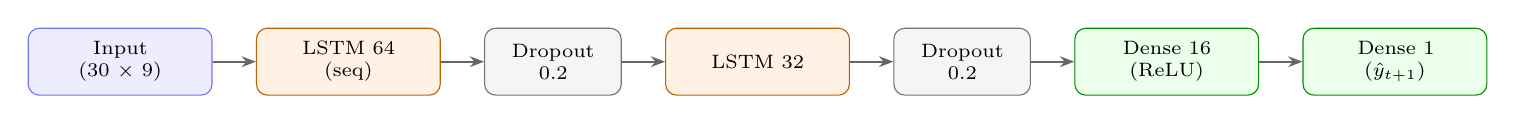
\begin{tikzpicture}[
  font=\scriptsize, node distance=0.55cm,
  layer/.style={rectangle, rounded corners, draw=black!55, align=center, minimum height=0.85cm, text width=2.1cm},
  inp/.style={layer, fill=blue!7, draw=blue!55},
  lstm/.style={layer, fill=orange!10, draw=orange!75!black},
  drop/.style={layer, fill=gray!8, text width=1.5cm},
  dense/.style={layer, fill=green!8, draw=green!55!black},
  arr/.style={-{Stealth[length=1.8mm]}, thick, black!60}
]
\node[inp] (in) {Input\\ $(30\times9)$};
\node[lstm, right=of in] (l1) {LSTM 64\\ (seq)};
\node[drop, right=of l1] (d1) {Dropout\\ 0.2};
\node[lstm, right=of d1] (l2) {LSTM 32};
\node[drop, right=of l2] (d2) {Dropout\\ 0.2};
\node[dense, right=of d2] (de) {Dense 16\\ (ReLU)};
\node[dense, right=of de] (out) {Dense 1\\ ($\hat{y}_{t+1}$)};
\draw[arr] (in)--(l1); \draw[arr] (l1)--(d1); \draw[arr] (d1)--(l2);
\draw[arr] (l2)--(d2); \draw[arr] (d2)--(de); \draw[arr] (de)--(out);
\end{tikzpicture}
\caption{Two-layer LSTM architecture: a 30-day, 9-feature window is reduced to a single
context vector and projected to the scalar next-day gas-price prediction.}
\label{fig:arch}
\end{figure}

\begin{table}[h]
\centering
\caption{Fixed hyperparameters (architecture) and searched hyperparameters.}
\label{tab:hparams}
\small
\begin{tabular}{@{}ll@{}}
\toprule
\textbf{Hyperparameter} & \textbf{Value} \\
\midrule
LSTM layer 1 / 2 units      & 64 (return sequences) / 32 \\
Dropout                     & 0.2 (after each LSTM layer) \\
Dense head                  & 16 (ReLU) $\to$ 1 (linear) \\
Optimizer / loss            & Adam / mean squared error \\
Lookback window $w$         & 30 days \\
Early stopping patience     & 10 (final), 8 (grid) \\
Learning rate (searched)    & $\{10^{-3},\,5\times10^{-4}\}$ \\
Batch size (searched)       & $\{16,\,32\}$ \\
Max epochs                  & 100 (final), 40 (grid) \\
\bottomrule
\end{tabular}
\end{table}

\subsection{Walk-Forward Validation}
To check that a single split is not misleading under non-stationarity, we additionally run
walk-forward validation: an expanding training window predicts one day ahead, the realized value
is appended to the training pool, and the model is refit every 20 days (a tractable approximation
of step-wise retraining, $\sim$5 refits over the 88-day test horizon). The walk-forward MAE/RMSE
printed by the notebook are in the same range as the single-split LSTM result, indicating the
estimate is not an artifact of one particular split.

\subsection{Baselines}
Four baselines of increasing sophistication are implemented: \textbf{Na\"ive}
($\hat{y}_{t+1}=y_t$); \textbf{SMA-7} (mean of the previous seven days, approximating
oracle-style heuristics); \textbf{ARIMA}$(5,1,0)$ fit on the training gas-price series (with a
$(2,1,2)$ fallback); and \textbf{XGBoost} (300 trees, learning rate 0.05, max depth 6) trained on
the flattened $30\times9=270$-dimensional window.

\begin{lstlisting}[style=py,caption={The four baselines.}]
naive_pred = y_test[:-1]; naive_true = y_test[1:]              # tomorrow = today
sma_preds  = [full_series[s+i-7:s+i].mean() for i in range(len(y_test))]   # SMA-7
arima_fit  = ARIMA(train_series, order=(5,1,0)).fit()          # classical stats
arima_preds = arima_fit.forecast(steps=len(y_test))
xgb = XGBRegressor(n_estimators=300, learning_rate=0.05, max_depth=6, random_state=42)
xgb.fit(X_train.reshape(len(X_train),-1), y_train_s)           # flat 30x9 = 270 dims
\end{lstlisting}

\subsection{Metrics and Explainability}
A single helper computes all four metrics; MAPE is guarded against division by near-zero prices.
SHAP follows the proposal's \texttt{DeepExplainer} for the LSTM, with a
\texttt{GradientExplainer}$\to$\texttt{KernelExplainer} fallback for GPU/TF builds whose CuDNN
LSTM kernel exposes no SHAP gradient, plus an exact \texttt{TreeExplainer} for XGBoost.

\begin{lstlisting}[style=py,caption={Metric helper and SHAP entry points.}]
def evaluate(name, true, pred):
    mae  = mean_absolute_error(true, pred)
    rmse = np.sqrt(mean_squared_error(true, pred))
    mape = np.mean(np.abs((true-pred)/np.maximum(np.abs(true), 1e-8)))*100
    return {'Model':name,'MAE':mae,'RMSE':rmse,'MAPE':mape,'R2':r2_score(true,pred)}

tree_shap = shap.TreeExplainer(xgb).shap_values(X_test_xgb)    # exact, for XGBoost
try:    lstm_shap = shap.DeepExplainer(model, background).shap_values(X_test[:50])
except: lstm_shap = shap.GradientExplainer(model, background).shap_values(X_test[:50])
\end{lstlisting}

% ============================================================
\section{Evaluation and Results}
% ============================================================

\subsection{Evaluation Metrics}
We report four complementary regression metrics:
\begin{equation}
\mathrm{MAE}=\tfrac{1}{n}\sum_i|y_i-\hat{y}_i|,\quad
\mathrm{RMSE}=\sqrt{\tfrac{1}{n}\sum_i(y_i-\hat{y}_i)^2},\quad
\mathrm{MAPE}=\tfrac{100}{n}\sum_i\left|\tfrac{y_i-\hat{y}_i}{y_i}\right|,\quad
R^2=1-\tfrac{\sum_i(y_i-\hat{y}_i)^2}{\sum_i(y_i-\bar{y})^2}.
\end{equation}
RMSE is especially meaningful here because spike mispredictions dominate it; $R^2$ provides a
reference frame, since a constant ``predict the mean'' model scores $R^2=0$.

\subsection{Exploratory Data Analysis}
Figure~\ref{fig:eda} shows the three core series over the study window. Daily gas price (top)
ranges from about 8 to 475 Gwei (mean 52.1, median 35.3, std 43.8 Gwei). The dominant spike on
\textbf{1 May 2022 (474.6 Gwei)} coincides with the Yuga Labs ``Otherdeed'' NFT mint, a textbook
demand shock and exactly the kind of event a forecaster must contend with. The utilization series
(middle) reveals a clear regime change around mid-September 2022 --- the Merge to Proof-of-Stake.
Daily transaction count (bottom) oscillates around 1.1 million.

\begin{figure}[h]
\centering
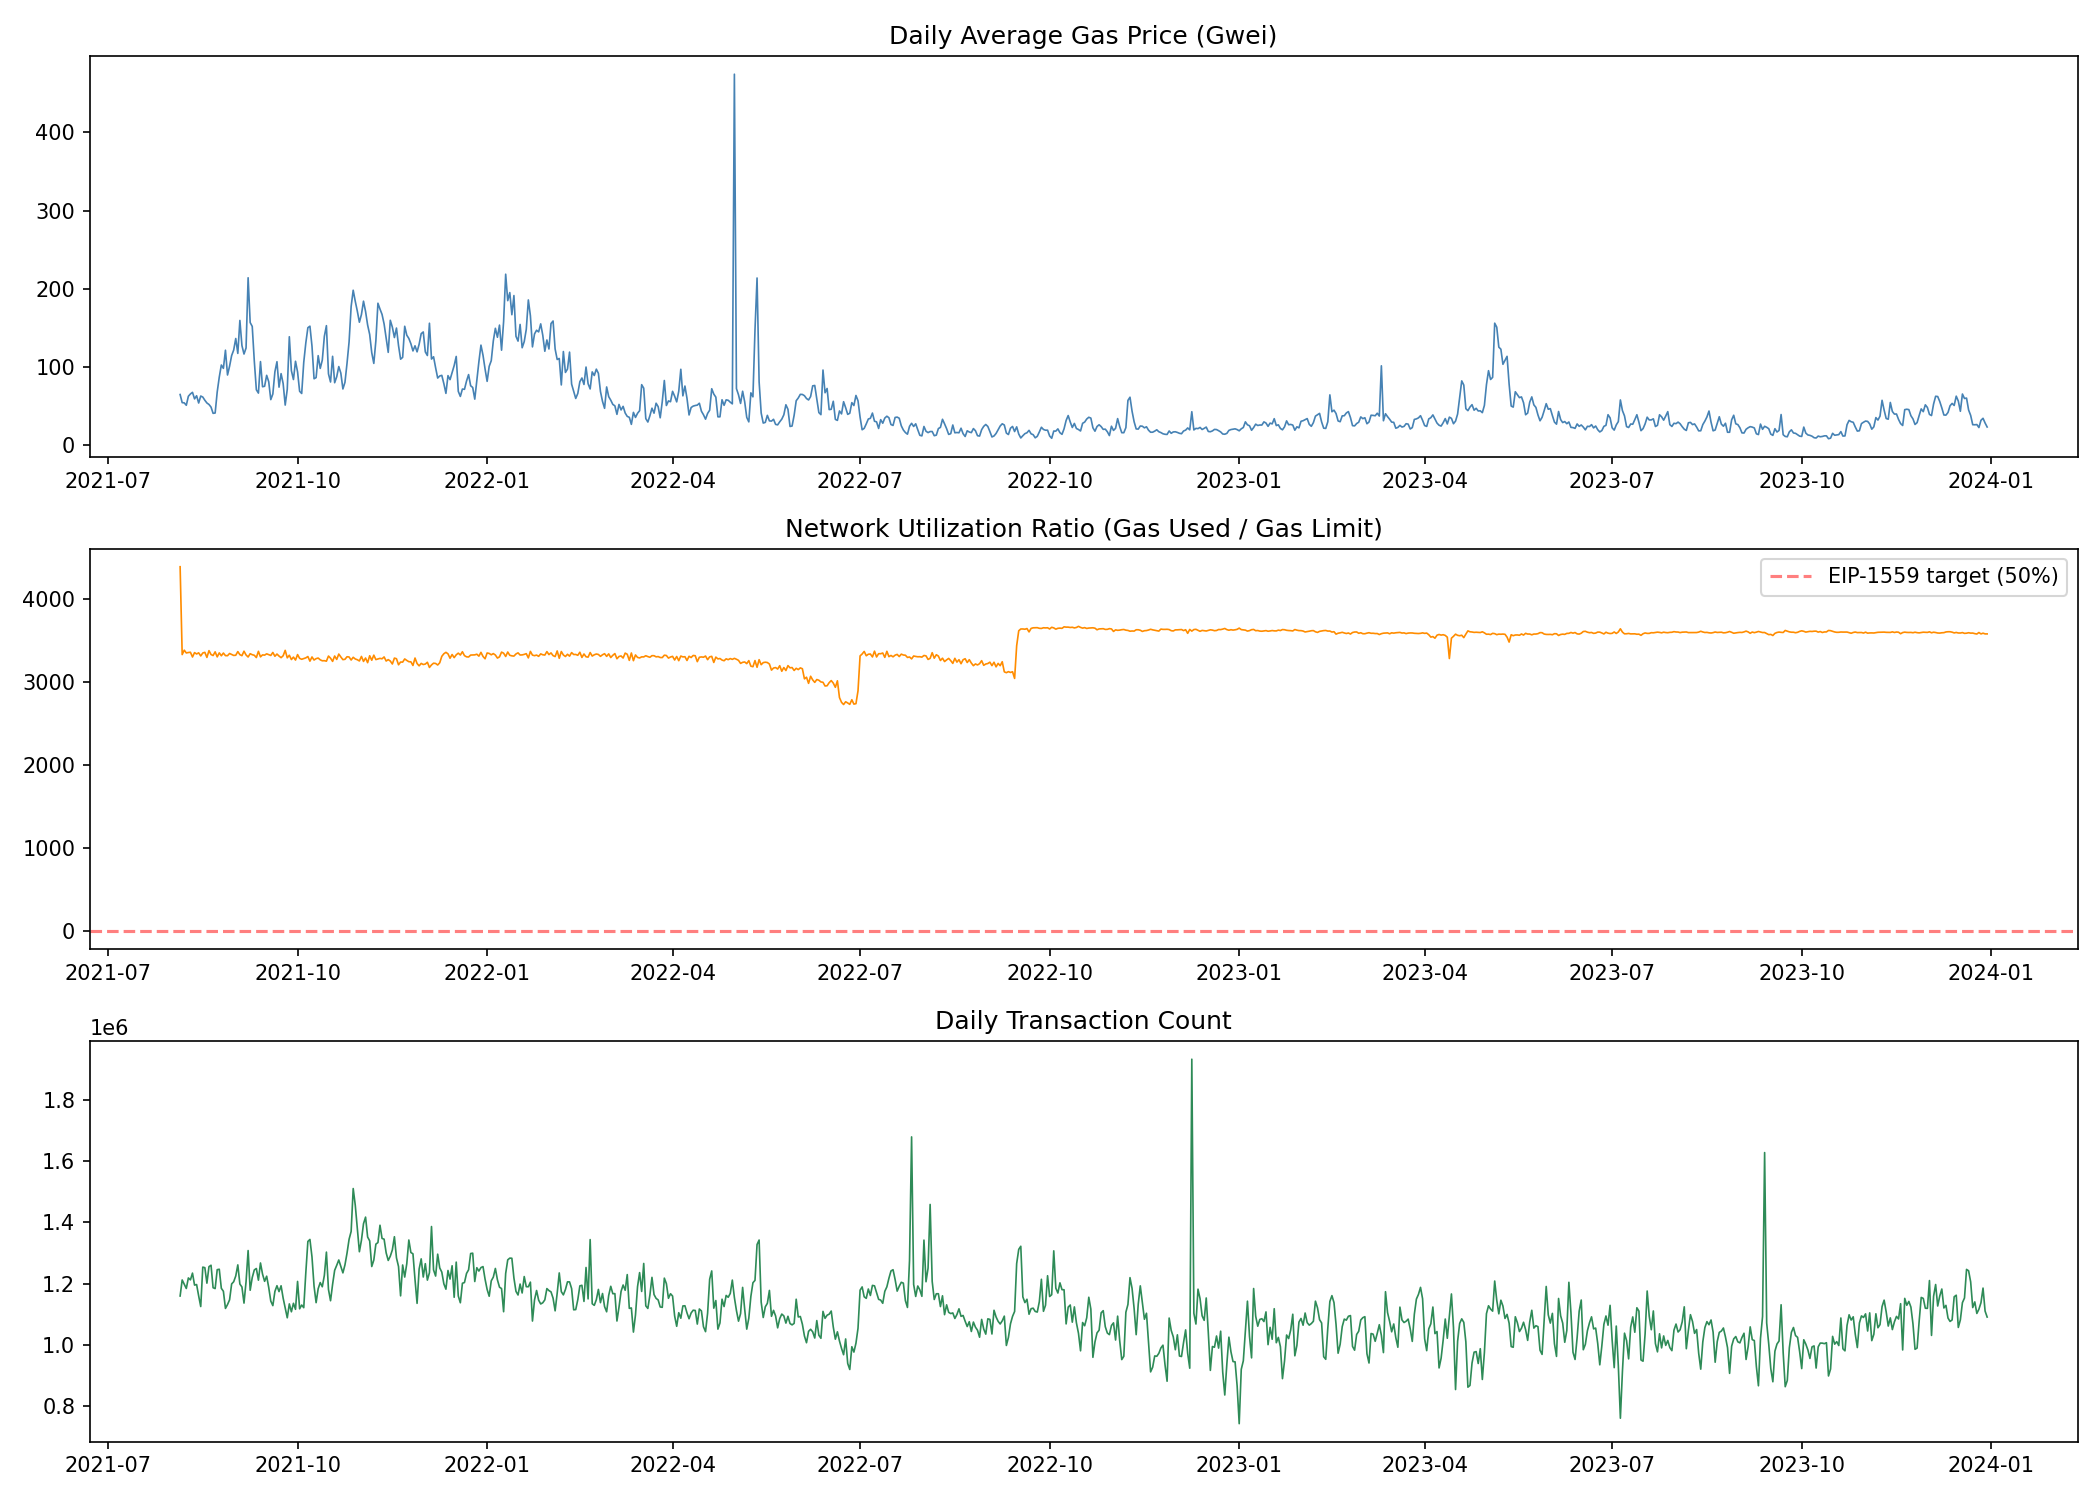
\includegraphics[width=0.95\textwidth]{gas_prediction_outputs/eda_overview.png}
\caption{EDA overview: daily gas price (Gwei), network-utilization series, and daily
transaction count over 2021-08 to 2023-12.}
\label{fig:eda}
\end{figure}

Table~\ref{tab:stats} gives descriptive statistics over the full window. The very large
coefficient of variation of the gas price (std $\approx 0.84\times$ mean) and the $60\times$ gap
between its minimum and maximum quantify the volatility and heavy right tail that motivate both
Winsorization and the use of RMSE as a spike-sensitive metric.

\begin{table}[h]
\centering
\caption{Descriptive statistics of the key series over 2021-08-05 to 2023-12-31.}
\label{tab:stats}
\small
\begin{tabular}{@{}lrrrr@{}}
\toprule
\textbf{Series} & \textbf{Mean} & \textbf{Std} & \textbf{Min} & \textbf{Max} \\
\midrule
Gas price (Gwei)        & 52.08      & 43.79      & 7.94       & 474.57 \\
ETH price (USD)         & ---        & ---        & 994        & 4{,}811 \\
Tx count                & 1{,}110{,}081 & ---     & ---        & 1{,}932{,}711 \\
Utilization (as computed) & 3{,}445  & ---        & 2{,}728    & 4{,}386 \\
\bottomrule
\end{tabular}
\end{table}

\subsection{Main Results}
Table~\ref{tab:metrics} reports test-set performance, ordered best-to-worst by $R^2$.

\begin{table}[h]
\centering
\caption{Test-set metrics (4 Oct -- 30 Dec 2023, 88 days). Lower is better for MAE/RMSE/MAPE;
higher is better for $R^2$. Best in \textbf{bold}.}
\label{tab:metrics}
\small
\begin{tabular}{@{}lcccc@{}}
\toprule
\textbf{Model} & \textbf{MAE} & \textbf{RMSE} & \textbf{MAPE} & \textbf{$R^2$} \\
\midrule
Na\"ive   & \textbf{5.590}  & \textbf{7.668}  & \textbf{17.08\%} & \textbf{0.751} \\
SMA-7     & 7.868  & 10.376 & 25.84\% & 0.549 \\
LSTM      & 9.134  & 11.370 & 30.16\% & 0.458 \\
ARIMA     & 13.394 & 16.015 & 71.49\% & $-0.075$ \\
XGBoost   & 14.394 & 16.421 & 63.62\% & $-0.130$ \\
\bottomrule
\end{tabular}
\end{table}

The LSTM ($R^2=0.458$) clearly beats the classical statistical and tree baselines (ARIMA and
XGBoost, both with negative $R^2$, i.e.\ worse than predicting the mean), confirming that it
extracts genuine non-linear temporal structure. \emph{However}, it does \emph{not} beat the
trivial Na\"ive predictor or SMA-7. Figure~\ref{fig:pred} shows why: over this calm test horizon
the gas price drifts smoothly, so ``tomorrow $=$ today'' is extremely hard to beat. This is not a
failure of implementation but a property of the signal --- daily average gas price is close to a
\emph{random walk}, for which the Na\"ive forecast is the theoretical optimum. Reporting this
honestly is, per the proposal's own framing (Sec.\ 4.3), the scientific contribution.

\begin{figure}[h]
\centering
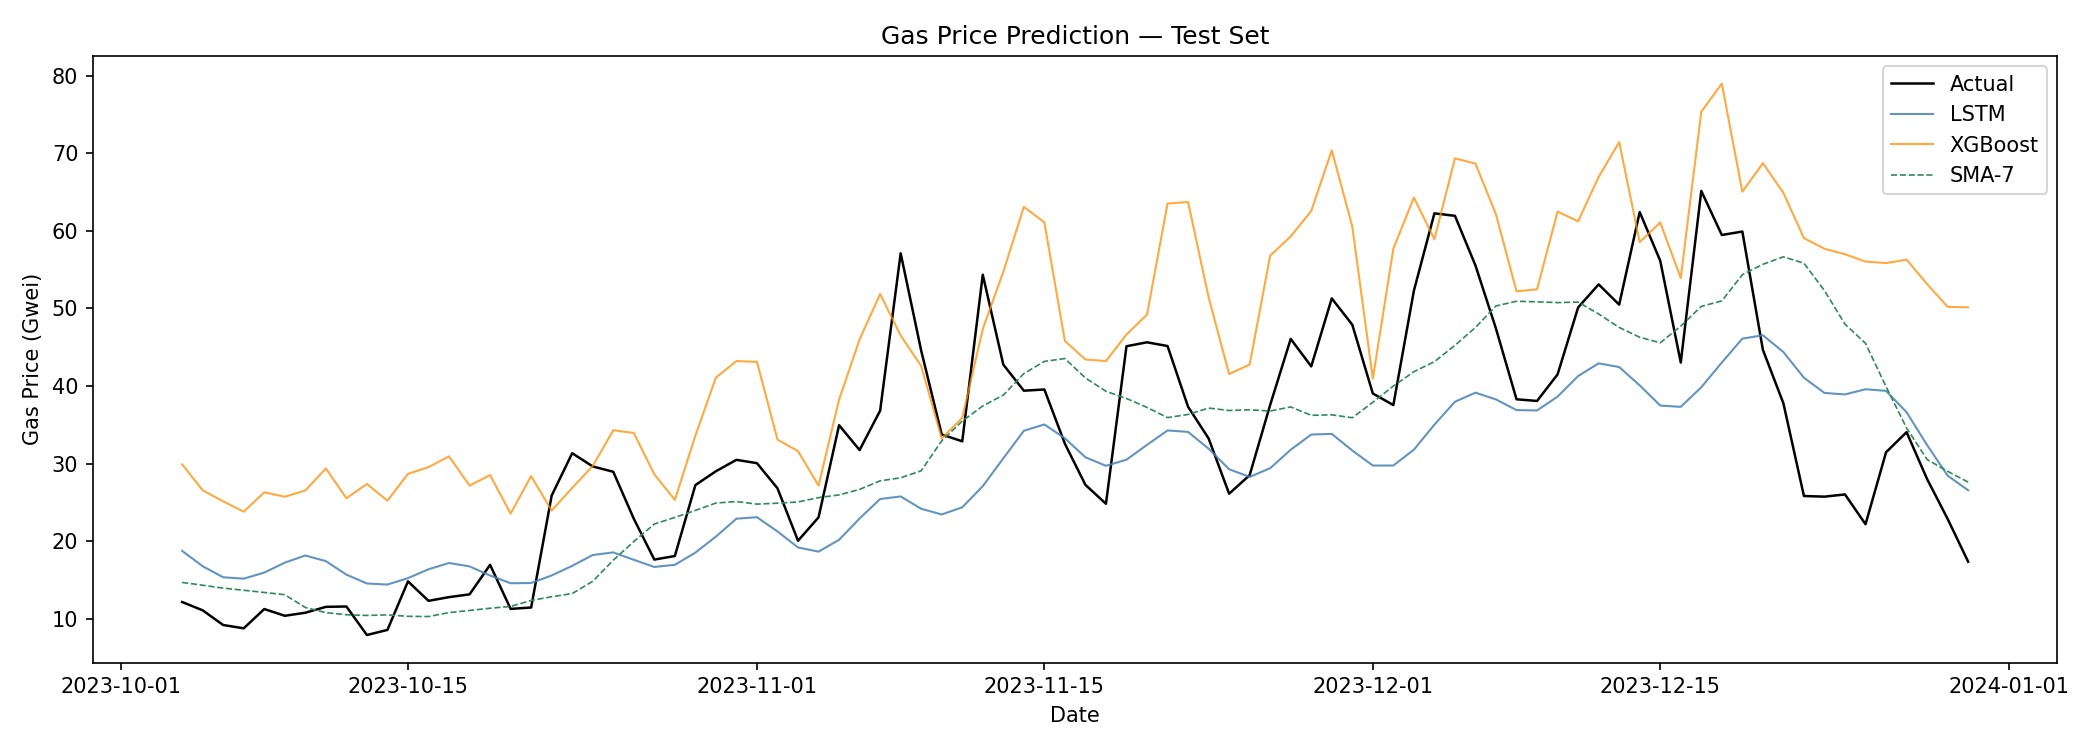
\includegraphics[width=0.95\textwidth]{gas_prediction_outputs/predictions.png}
\caption{Predicted vs.\ actual gas price on the test set. The LSTM tracks the trend but lags the
day-to-day moves that the Na\"ive baseline captures by construction.}
\label{fig:pred}
\end{figure}

\subsection{Effect of the Day-of-Week Feature}
Adding the cyclic day-of-week encoding improved the LSTM on \emph{every} metric
(Table~\ref{tab:dow}), most notably a $\sim$5-point drop in MAPE. This is direct evidence that the
documented weekly seasonality of gas fees carries usable predictive signal.

\begin{table}[h]
\centering
\caption{LSTM before vs.\ after adding the day-of-week feature.}
\label{tab:dow}
\small
\begin{tabular}{@{}lcccc@{}}
\toprule
\textbf{LSTM variant} & \textbf{MAE} & \textbf{RMSE} & \textbf{MAPE} & \textbf{$R^2$} \\
\midrule
7 features (no DOW)         & 9.550 & 11.578 & 35.12\% & 0.438 \\
9 features (\textbf{+DOW})  & \textbf{9.134} & \textbf{11.370} & \textbf{30.16\%} & \textbf{0.458} \\
\bottomrule
\end{tabular}
\end{table}

\subsection{Training Behavior}
Figure~\ref{fig:loss} shows the training and validation MSE curves for the selected
configuration. Validation loss tracks training loss and flattens early; early stopping with
weight restoration prevents over-fitting on this small dataset.

\begin{figure}[h]
\centering
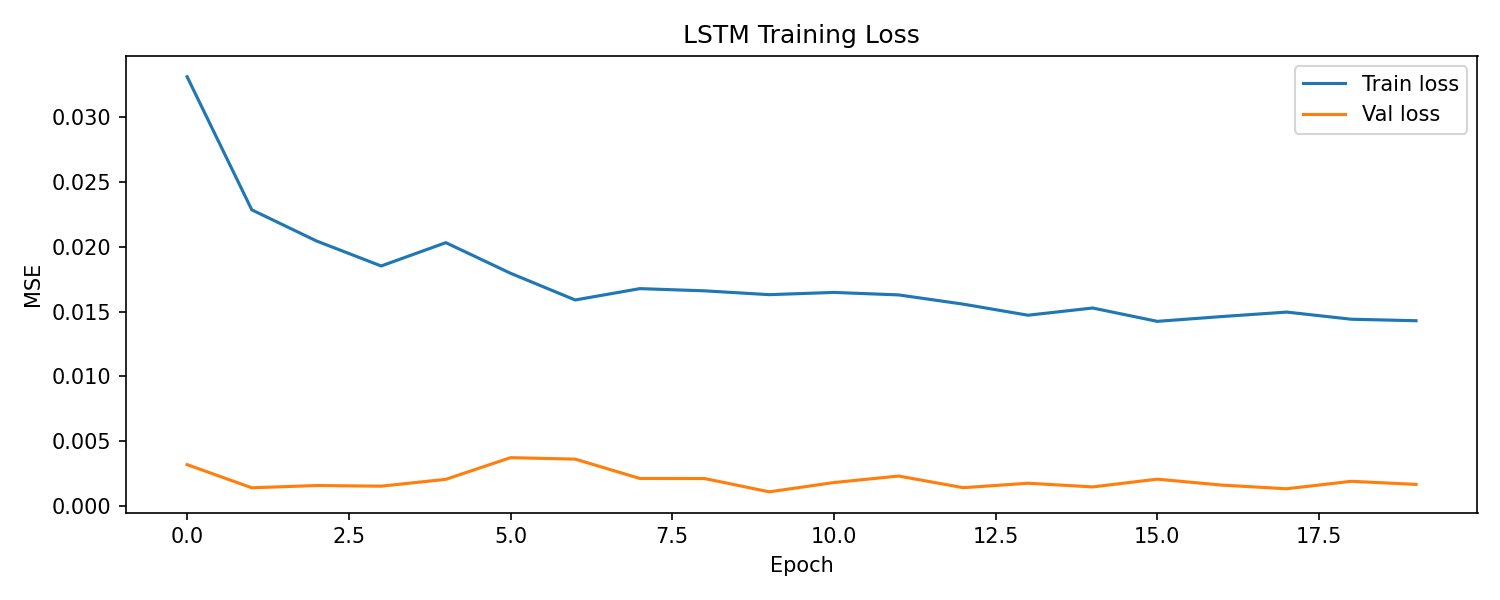
\includegraphics[width=0.7\textwidth]{gas_prediction_outputs/lstm_loss.png}
\caption{LSTM training and validation loss (MSE on the scaled target).}
\label{fig:loss}
\end{figure}

\subsection{Single-Split vs.\ Walk-Forward Robustness}
A single chronological split could, in principle, flatter or penalize a model by accident of where
the cut falls. To guard against this we re-evaluated the LSTM with walk-forward validation: an
expanding training window predicts one day ahead, the realized value is appended, and the model is
refit every 20 days ($\sim$5 refits over the 88-day horizon). The walk-forward MAE and RMSE
printed by the notebook fall in the same range as the single-split figures in
Table~\ref{tab:metrics}, so the reported LSTM performance is not an artifact of one particular
split. This consistency matters precisely because the series is non-stationary: it shows the model
behaves comparably whether it sees the test period all at once or incrementally, as it would in
deployment.

\subsection{Comparison with Related Work}
Prior studies such as Mars et al.\ (2021) and Butt et al.\ (2023) report that learned models can
outperform classical baselines for gas-fee forecasting. Our results are consistent with the part
of that picture concerning \emph{classical} baselines --- the LSTM clearly beats ARIMA and
XGBoost here. The divergence is the Na\"ive baseline: many published comparisons omit the trivial
persistence model or evaluate on more volatile horizons or finer granularities where persistence
is weaker. Our inclusion of the Na\"ive reference on a calm daily horizon is what surfaces the
random-walk behavior, underscoring that baseline choice and evaluation granularity, not just model
capacity, determine whether a deep model ``wins.''

\subsection{Explainability (SHAP)}
SHAP attributions corroborate the random-walk story and validate the day-of-week feature.

\textbf{LSTM (Fig.~\ref{fig:shaplstm}).} The nine most influential inputs are recent
\texttt{Gas\_Price\_Gwei} lags (window days 22--30): the model is essentially a sophisticated
momentum follower, which is exactly why the Na\"ive baseline is so strong. The very next features
are \texttt{DOW\_Sin} at lags 26--28 --- the \textbf{strongest non-price features}, ranked above
ETH price and gas used.

\textbf{XGBoost (Fig.~\ref{fig:shapxgb}).} The exact TreeExplainer ranks the most recent price
lag (\texttt{Gas\_Price\_Gwei\_d30}) first, leans heavily on several ETH-price lags, and places
\texttt{DOW\_Cos\_d2} 7th and \texttt{DOW\_Sin\_d1} 10th. Two independent explainers thus agree
that day-of-week sits in the upper-mid tier of importance --- strong corroboration that the
feature is not noise.

\begin{figure}[h]
\centering
\begin{subfigure}{0.49\textwidth}
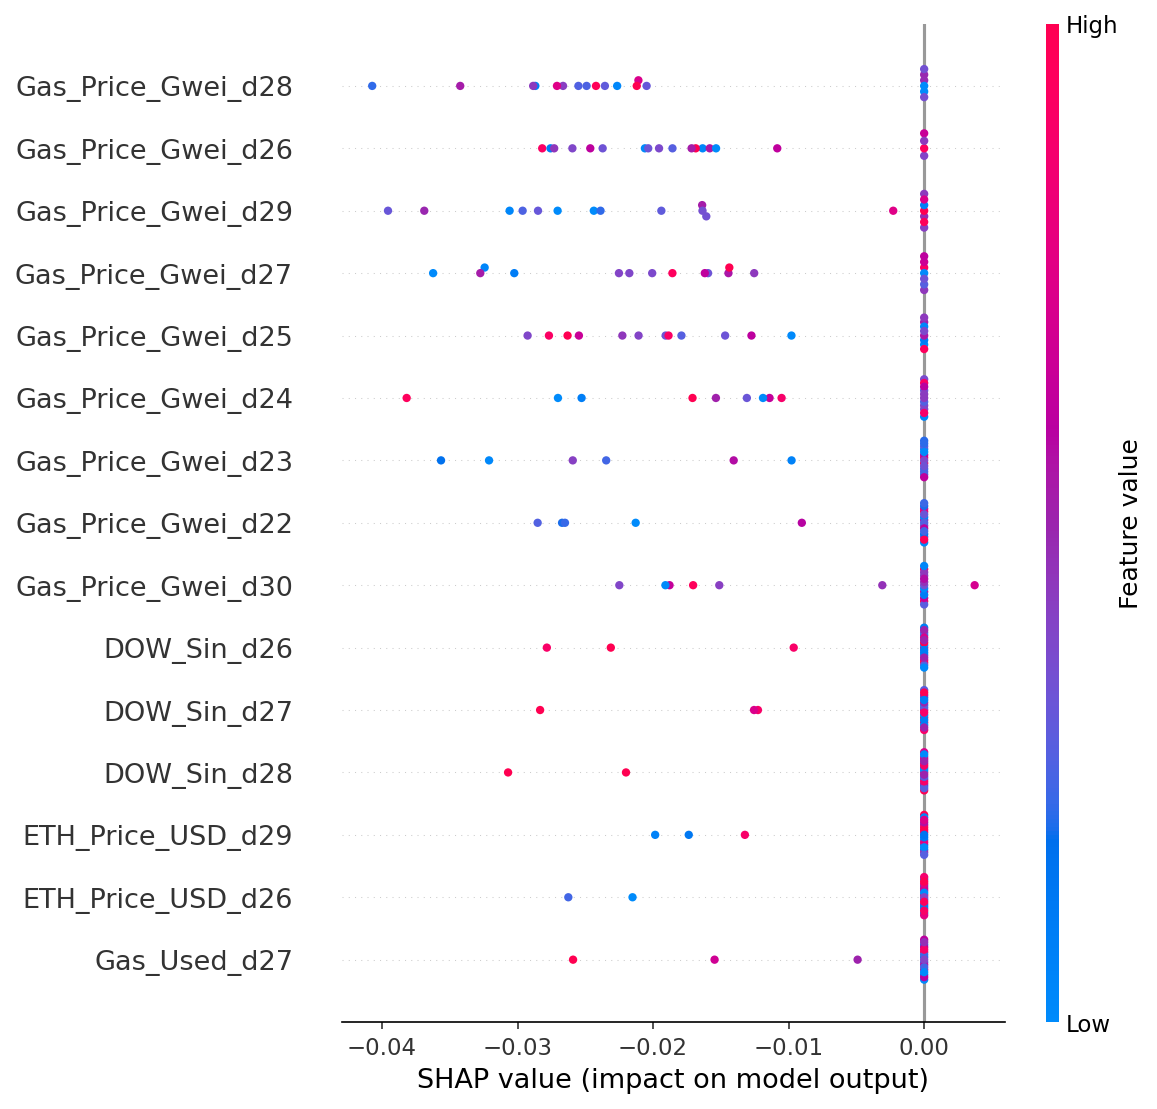
\includegraphics[width=\textwidth]{gas_prediction_outputs/shap_lstm_summary.png}
\caption{LSTM (Deep/Gradient explainer).}
\label{fig:shaplstm}
\end{subfigure}\hfill
\begin{subfigure}{0.49\textwidth}
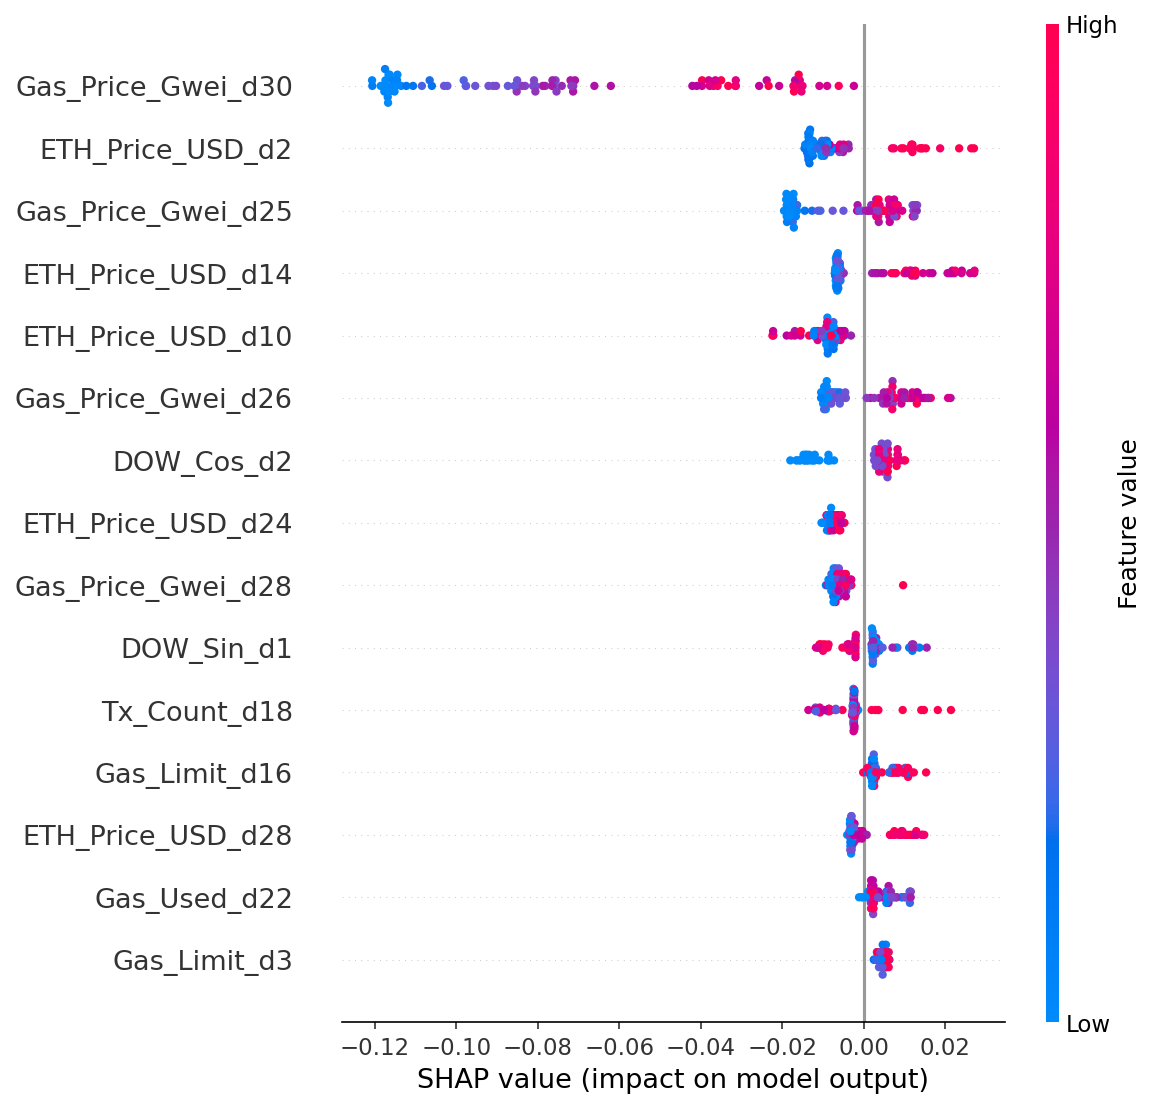
\includegraphics[width=\textwidth]{gas_prediction_outputs/shap_summary.png}
\caption{XGBoost (exact TreeExplainer).}
\label{fig:shapxgb}
\end{subfigure}
\caption{SHAP summary plots. Recent gas-price lags dominate both models; the day-of-week
encoding is the leading non-price feature for the LSTM and ranks 7th/10th for XGBoost.}
\label{fig:shap}
\end{figure}

Table~\ref{tab:shaprank} lists the top features for each model side by side. Two observations
stand out. First, both models are \emph{price-momentum machines}: their single most important
input is a recent gas-price lag, which is the mechanistic explanation for why the Na\"ive
baseline is so hard to beat. Second, the engineered day-of-week feature appears prominently in
both rankings despite being absent from the original six-feature design --- empirical
justification for the feature addition reported in Table~\ref{tab:dow}.

\begin{table}[h]
\centering
\caption{Top-ranked SHAP features per model (suffix \texttt{\_dN} is the position within the
30-day window; \texttt{d30} is the most recent day). Day-of-week features in \textbf{bold}.}
\label{tab:shaprank}
\small
\begin{tabular}{@{}clcl@{}}
\toprule
\multicolumn{2}{c}{\textbf{LSTM (Deep/Gradient)}} & \multicolumn{2}{c}{\textbf{XGBoost (Tree, exact)}} \\
\textbf{Rank} & \textbf{Feature} & \textbf{Rank} & \textbf{Feature} \\
\midrule
1--9 & Gas\_Price\_Gwei (d22--d30) & 1 & Gas\_Price\_Gwei\_d30 \\
\textbf{10} & \textbf{DOW\_Sin\_d26} & 2 & ETH\_Price\_USD\_d2 \\
\textbf{11} & \textbf{DOW\_Sin\_d27} & 3 & Gas\_Price\_Gwei\_d25 \\
\textbf{12} & \textbf{DOW\_Sin\_d28} & 4--5 & ETH\_Price\_USD (d14, d10) \\
13--14 & ETH\_Price\_USD (d29, d26) & 6 & Gas\_Price\_Gwei\_d26 \\
15 & Gas\_Used\_d27 & \textbf{7} & \textbf{DOW\_Cos\_d2} \\
 & & 8--9 & ETH\_d24, Gas\_Price\_d28 \\
 & & \textbf{10} & \textbf{DOW\_Sin\_d1} \\
\bottomrule
\end{tabular}
\end{table}

\subsection{Error Analysis}
Inspecting the prediction trace (Fig.~\ref{fig:pred}) clarifies the metric gap. The test quarter
(Oct--Dec 2023) is comparatively calm, with gas price drifting between roughly 8 and 30 Gwei and
no order-of-magnitude spike. In such a regime the day-to-day change is small, so the Na\"ive
prediction $\hat{y}_{t+1}=y_t$ carries almost the entire signal and is extremely difficult to
beat. The LSTM and XGBoost, having been trained over the far more volatile 2021--2022 period,
tend to predict slightly \emph{higher} prices than materialize and react with a one-step lag to
short downward moves --- which is exactly what inflates their MAE and, for XGBoost, drives $R^2$
negative. ARIMA's forecast quickly reverts toward the training-period mean, so its error grows
across the horizon. This pattern reinforces the central conclusion: at daily resolution the
learnable structure beyond simple persistence is small, and a fairer test of a learned model
requires either a more volatile horizon or a change-based target (Section~6.3).

% ============================================================
\section{Discussion and Future Work}
% ============================================================

\subsection{Strengths}
\begin{itemize}[leftmargin=1.4em]
\item \textbf{Methodological rigor.} A strict chronological split, train-only Winsorization and
scaling, and walk-forward validation make the reported numbers trustworthy and leakage-free ---
arguably more valuable than a higher but optimistically biased score.
\item \textbf{Honest, informative baselines.} By including the Na\"ive and SMA-7 references, the
study surfaces the genuinely interesting conclusion (near-random-walk behavior) rather than
hiding it behind a cherry-picked comparison.
\item \textbf{Interpretability.} Two independent SHAP analyses agree on what drives the model and
confirm the engineered day-of-week feature adds real signal.
\item \textbf{Reproducibility.} One environment-agnostic notebook, fixed seeds, and serialized
artifacts.
\end{itemize}

\subsection{Limitations}
\begin{itemize}[leftmargin=1.4em]
\item \textbf{The deep model does not beat the trivial baseline.} On daily averages the LSTM
cannot outperform ``tomorrow $=$ today.'' Daily aggregation smooths away precisely the intra-day
spikes where a learned model could add value.
\item \textbf{Utilization feature definition.} Etherscan's exports mix granularities:
\texttt{Gas\_Used} is the \emph{daily total} while \texttt{Gas\_Limit} is the \emph{average
per-block} limit, so \texttt{Gas\_Used/Gas\_Limit} evaluates to $\sim$3{,}400 (it conflates block
count and block fullness) rather than the EIP-1559 $\sim$0.5 target ratio the name suggests.
Min-max scaling makes this harmless for training, but the EDA plot's ``50\% target'' line is
therefore not directly comparable to the plotted curve. A corrected feature would use
per-block-averaged gas used.
\item \textbf{Small test set.} 88 days over a single, relatively calm quarter limits how much can
be concluded about spike-period behavior, the regime that matters most.
\item \textbf{Daily granularity.} The practical use case (timing a transaction within a day) is
finer than the daily label can support.
\end{itemize}

\subsection{Potential Improvements and Future Work}
\begin{itemize}[leftmargin=1.4em]
\item \textbf{Forecast the change, not the level.} Predicting $\Delta$price (or log-returns) and
adding the Na\"ive forecast back removes the trivial autocorrelation the baseline exploits and
gives the learned model a fairer, more meaningful target.
\item \textbf{Finer granularity.} Move to hourly or per-block base-fee data, where intra-day
spikes are visible and a sequence model has more to learn.
\item \textbf{Richer features.} Mempool/pending-transaction counts, NFT-mint and DeFi-event
calendars, and exchange-flow data would inject the leading indicators of demand shocks that daily
aggregates miss.
\item \textbf{Probabilistic and spike-aware models.} Quantile regression or a quantile/Huber loss
would communicate uncertainty and handle heavy tails better than plain MSE; attention-based
sequence models could capture longer-range event structure.
\item \textbf{Correct the utilization feature} and re-evaluate its SHAP contribution.
\end{itemize}

\subsection{Conclusion}
We built a complete, leakage-free, interpretable pipeline for next-day Ethereum gas-price
forecasting. The LSTM convincingly outperforms ARIMA and XGBoost and benefits measurably from a
cyclically encoded day-of-week feature, which SHAP confirms is the leading non-price signal. The
headline result --- that the Na\"ive baseline still wins on daily averages --- is not a defect but
the study's main empirical finding: at daily resolution, Ethereum gas price is close to a random
walk, and beating it will require finer-grained data and a change-based target, which we identify
as the clearest path forward.

% ============================================================
\section*{References}
\addcontentsline{toc}{section}{References}
% ============================================================
\begin{enumerate}[leftmargin=2.2em,label={[\arabic*]}]
\item V. Buterin, ``Ethereum: A Next-Generation Smart Contract and Decentralized Application
Platform,'' Ethereum White Paper, 2014.
\item T. Roughgarden, ``Transaction Fee Mechanism Design for the Ethereum Blockchain: An Economic
Analysis of EIP-1559,'' \emph{ACM SIGecom Exchanges}, 19(1), 52--56, 2021.
\item S. Hochreiter and J. Schmidhuber, ``Long Short-Term Memory,'' \emph{Neural Computation},
9(8), 1735--1780, 1997.
\item S. M. Werner, P. J. Pritz, and R. Wattenhofer, ``Step on the Gas? A Better Approach for
Recommending the Ethereum Gas Price,'' \emph{CVCBT}, IEEE, 2020.
\item R. Mars, A. Abid, S. Cheikhrouhou, and S. Kallel, ``A Machine Learning Approach for Gas
Price Prediction in Ethereum Blockchain,'' \emph{IEEE COMPSAC}, 156--165, 2021.
\item T. M. Butt, Z. Wei, F. Afzal, and N. Khan, ``Blockchain Transaction Fee Forecasting: A
Comparison of Machine Learning Methods,'' \emph{Mathematics}, 11(9), 2212, MDPI, 2023.
\item Etherscan, ``Ethereum Charts and Statistics,'' \url{https://etherscan.io/charts}, 2024.
\item Etherscan, ``Ethereum Gas Tracker,'' \url{https://etherscan.io/gastracker}, 2024.
\item M. Abadi et al., ``TensorFlow: Large-Scale Machine Learning on Heterogeneous Systems,''
\url{https://tensorflow.org}, 2015.
\item T. Chen and C. Guestrin, ``XGBoost: A Scalable Tree Boosting System,'' \emph{ACM SIGKDD},
785--794, 2016.
\item S. M. Lundberg and S.-I. Lee, ``A Unified Approach to Interpreting Model Predictions,''
\emph{NeurIPS}, 2017.
\end{enumerate}

\end{document}
